Applying Feature Selection techniques to medical data such as clinical, genomic, proteomic or metabolomic information could solve two important medical problems. One is related to the task of finding which are the relevant variables involved in a disease, response to treatment, survival time, relapse probability, etc. It could lead to understand better the disease mechanisms, evaluate the factors that are involved or even propose new hypotheses about factors that have not been taken into account until this moment. The second one is to perform variable reduction and learn a predictive model with the best possible performance to cost ratio by using the minimum set of diagnostic variables. This estimator could then be used as an aid in clinical decisions or as an indicator for research. In this case, the focus can be moved from the relevancy of the reduced variable subset to the final performance of the model. 
\\

Despite the considerable efforts made in capturing health data, the common situation is still having much more variables than observations (individuals). While the number of observations is usually around hundreds or thousands, the number of variables could reach millions. This is an unfavourable condition for any Machine Learning algorithm (Bellman's curse of dimensionality \cite{Bellman2015AdaptiveTour}). Ensemble feature selection received increasing attention during the last decade \cite{Bolon-Canedo2019EnsemblesTrends} \cite{Pes2020EnsembleDomains} and consists in combining the output of several inducers applied on distinct subset of a database. It results in an improvement of the selection stability and robustness to the lack of observations. Nevertheless, more work is required especially with relevant but redundant variables which tend not to be selected. 
\\

We'll be developing an algorithm which proposes a list of features that contribute to a better prediction of disease cases. The list of variables will be later forwarded to the expert team to be validated. 
There are no direct biological insights to be found, nor biomarkers to be discovered. Also, we study the behaviour of ensemble feature selection with redundant variables, interaction of which is commonly unknown and intricate to decipher.
\\

\subsection{Ensemble}
The inner construction of the Ensemble we used to perform this work is described in Figure \ref{fig:ensemble-diagram}.
\\

\begin{figure}[!htpb]
    \centering
    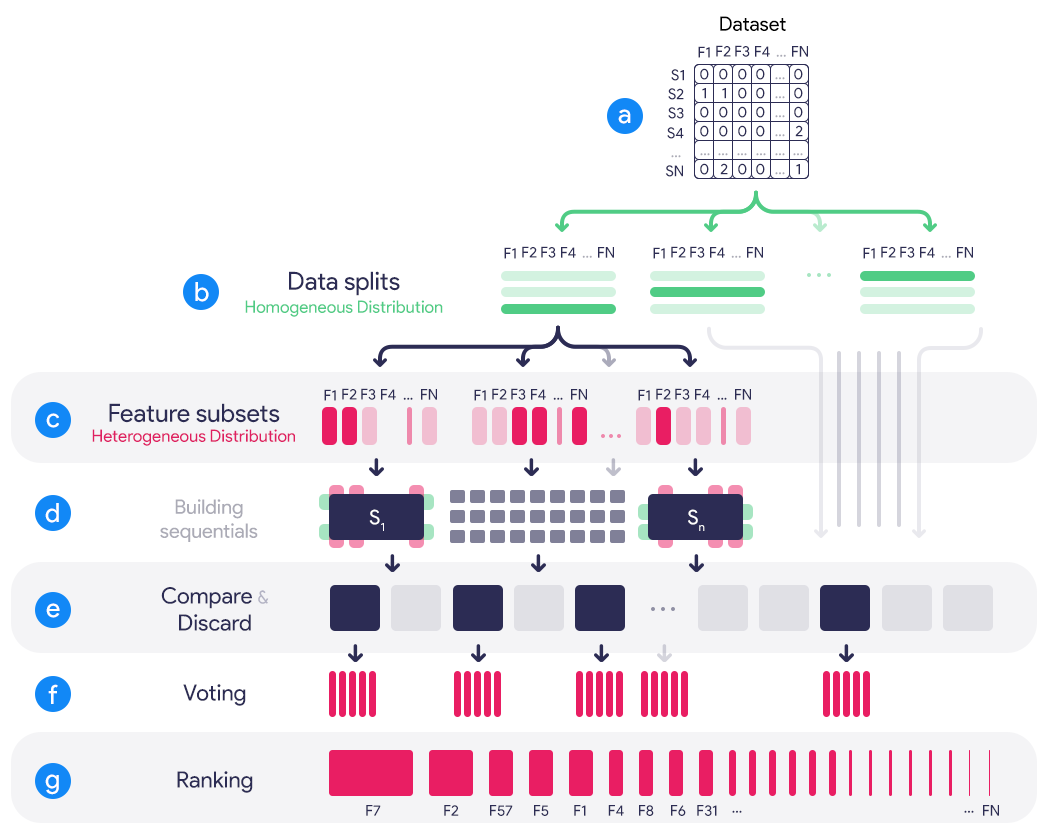
\includegraphics[width=\linewidth]{Major Thesis/figures/diagrams/Ensemble.png}
    \caption{Ensemble workflow}
    \label{fig:ensemble-diagram}
\end{figure}

A regular run of the algorithm has the following steps:
\begin{enumerate}
    \item Resample the data using a \emph{resampling without replacement} technique.
    \item Apply several feature selectors to each split, then evaluate their performance iteratively to achieve the best predictive variable subset. Each run delivers a \emph{sequential}.
    \item Discard sequentials which do not achieve an overall score above a set threshold.
    \item Aggregate sequentials results: Each feature appeareance in a sequential result adds a vote to the feature.
    \item Return the full list of features, discarding those not voted.
\end{enumerate}
\\

When an ensemble method attempts to assign votes to all variables, those features which hold a significant similarity might alternately receive the votes. E.g. assuming X and Y have a correlation of 0.99 and they obtain 5 and 10 votes respectively, their prediction might have been the same since they are highly similar at the eyes of the classifier. The total maximum of votes (15) has been split in two variables, and both have lost positions in the ranking. We name this phenomenon \emph{rivalry}.

Either highly redundant features (due to quasi-constant values, etc.) or features holding a strong rivalry hamper ensemble's aim to accurately rank variants.
\\

In this project we introduce an approach which performs an iterative swap between each of the variants in a feature set (already calculated in an individual sequential) and the missing features picked by the full ensemble (as a result of a consensus function) in order to perform a retraining of the sequentials and further compare the prediction results.
\\

In our definition of rivalry, two variables compete against each other with regard to a subset of variables if swapping them does not change the prediction.
More precisely, if the original prediction (A) and the set-swapped prediction (B), are similar more than a custom threshold (overlap(A, B) >= threshold), we consider the pair of features swapped are highly linked.
\\

Therefore, assessing one-to-one prediction similarity and investigating paired correlation allows us to re-rank the original ensemble output, helping us to tackle the vote rivalry problem.

% comment